\let\negmedspace\undefined
\let\negthickspace\undefined
\documentclass[journal]{IEEEtran}
\usepackage[a5paper, margin=10mm, onecolumn]{geometry}
%\usepackage{lmodern} % Ensure lmodern is loaded for pdflatex
\usepackage{tfrupee} % Include tfrupee package

\setlength{\headheight}{1cm} % Set the height of the header box
\setlength{\headsep}{0mm}     % Set the distance between the header box and the top of the text

\usepackage{gvv-book}
\usepackage{gvv}
\usepackage{cite}
\usepackage{amsmath,amssymb,amsfonts,amsthm}
\usepackage{algorithmic}
\usepackage{graphicx}
\usepackage{textcomp}
\usepackage{xcolor}
\usepackage{txfonts}
\usepackage{listings}
\usepackage{enumitem}
\usepackage{mathtools}
\usepackage{gensymb}
\usepackage{comment}
\usepackage[breaklinks=true]{hyperref}
\usepackage{tkz-euclide} 
\usepackage{listings}
% \usepackage{gvv}                                        
\def\inputGnumericTable{}                                 
\usepackage[latin1]{inputenc}                                
\usepackage{color}                                            
\usepackage{array}                                            
\usepackage{longtable}                                       
\usepackage{calc}                                             
\usepackage{multirow}                                         
\usepackage{hhline}                                           
\usepackage{ifthen}                                           
\usepackage{lscape}
\begin{document}

\bibliographystyle{IEEEtran}
\vspace{3cm}
\title{3.2.17}
\author{EE24BTECH11008 - Aslin Garvasis
}
% \maketitle
% \newpage
% \bigskip
{\let\newpage\relax\maketitle}

\renewcommand{\thefigure}{\theenumi}
\renewcommand{\thetable}{\theenumi}
\setlength{\intextsep}{10pt} % Space between text and floats
 \textbf{Question:}\\
 Constuct a triangle whose sides are $3.6cm, 3.0cm$ and $4.8cm.$ Bisect the smallest angle and measure each part.
 
 \solution \\ 
 \begin{table}[h!]    
  \centering
  \begin{tabular}[12pt]{ |c| c|}
    \hline
	\textbf{Variable}  & \textbf{Description} \\
    \hline
	$\vec{A}$$\brak{a,b}=\brak{8,9}$ &  coordinates of first point\\
    \hline 
	$\vec{B}$$\brak{-a,-b}=\brak{-8,-9}$ & coordinates of second point\\
    \hline
	$\vec{\brak{A-B}^T}\vec{\brak{A-B}}=\norm{\vec A-\vec B }^2$ &square of distance between $\vec A$ and $\vec B$\\  
    \hline
	$d$ & distance between $\vec A$ and $\vec B$\\
    \hline 	
         
\end{tabular}

  \caption{Input parameters}
  \label{tab1.1.9.16}
\end{table}
$\because$ The smallest angle is associated with the opposite smallest side.\\
The angle bisector of a triangle of a triangle divides the opposite side into two parts proportional to the other two sides of the triangle.\\
\begin{align}
	\because \norm{AC}&=3.6\\
	\because \norm{AB}&=4.8\\
	\because \norm{BC}&=3.0\\
	\cos{\angle BAC}&=\norm{\frac{\vec{AC}^T\vec{AB}}{\norm{AC}\norm{AB}}}=0.78\\
	\angle{BAC}&=38.73\degree\\
	\cos{\angle ABC}&=\norm{\frac{\vec{BC}^T\vec{BA}}{\norm{BC}\norm{BA}}}=0.66\\
	\angle{ABC}&=48.70\degree\\
	\cos{\angle ACB}&=\norm{\frac{\vec{CA}^T\vec{CB}}{\norm{CA}\norm{CB}}}=0.05
\end{align}
\begin{align}
	\angle{ACB}&=87.13\degree\\
	\therefore \vec{D}&=\frac{\norm{AC}.\vec{B}+\norm{AB}.\vec{C}}{\norm{AC}+\norm{BC}}\\
	\implies \vec{D}&=3.6\myvec{4.8\\0}+4.8\myvec{2.81\\2.24}=\myvec{3.66\\1.28}\\
	\cos{\angle BAD}&=\norm{\frac{\vec{AB}^T\vec{AD}}{\norm{AB}\norm{AD}}}=0.94\\
	\angle{BAD}&=19.28\degree\\
	\implies \norm{BD}&=\frac{\norm{BC}\norm{AB}}{\norm{AB}+\norm{AC}}=1.71\\
	\implies \norm{CD}&=\frac{\norm{BC}\norm{AC}}{\norm{AB}+\norm{AC}}=1.28
 \end{align}
 \newpage


		\begin{figure}[h!]
                \centering
               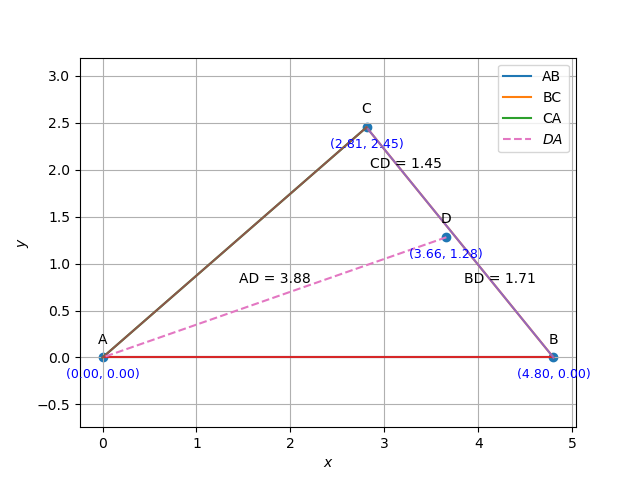
\includegraphics[width=0.7\linewidth]{figs/Fig1.png}
			\caption{Plot of points $\vec{A}$, $\vec{B}$, $\vec{C}$ and $\vec{D}$}
               
               \end{figure}
\end{document}
